\chapter{\heiti 软件使用}
\section{\heiti 打开控制软件}
进入我司为用户提供的“Integration”的文件夹,双击运行“ASG.py”文件,即可打开仪器控制软件。软件主界面(Pulse界面)如图4.1所示。
\begin{figure}[ht]
\centering
%\includegraphics[width=11cm,height=9cm]{fig4_1}
\includegraphics[height=9cm]{fig4_1}
\caption{软件主界面}
\end{figure}

在软件主界面中,每行8个绿色方框,从左往右依次代表OUT 1至OUT 8的8个方波输出通道在一段时间内的输出状态(时间长短由右侧的“Length”文本框内输入的数值决定,单位为纳秒)。当绿色被点亮时,该通道输出高电平;若绿色未被点亮,则该通道输出为低电平。

\section{\heiti 定义任意方波序列}
用户可根据每行绿色方框的不同状态及“Length”的长度来定义任意的方波序列。如用户想要在1、2、3、4通道生成一个高电平宽度为60 ns的方波序列,而5、6、7、8通道在这60 ns内为低电平。则可如图4.2 定义方波序列:
\begin{figure}[ht]
\centering
%\includegraphics[width=11cm,height=9cm]{fig4_2}
\includegraphics[height=9cm]{fig4_2}
\caption{自定义方波序列}
\end{figure}

\section{\heiti 定义方波序列注意事项}
\noindent \textbf{(1)}. 每个通道的方波序列中单个方波脉冲高低电平时间必须在7.5 ns至2.6 s以内。如用户定义的方波序列中存在单个脉冲宽度小于7.5 ns 的情况,则为非法输入,如图4.3。
\begin{figure}[H]
\centering
%\includegraphics[width=11cm,height=9cm]{fig4_3}
\includegraphics[height=9cm]{fig4_3}
\caption{宽度小于7.5 ns的非法方波序列输入}
\end{figure}

\newpage
\noindent \textbf{(2)}.  若用户定义的方波序列中存在单个脉冲宽度大于2.6 s的情况,亦为非法输入,如图4.4。
\begin{figure}[ht]
\centering
%\includegraphics[width=11cm,height=9cm]{fig4_4}
\includegraphics[height=9cm]{fig4_4}
\caption{宽度大于2.6 s的非法方波序列输入}
\end{figure}

\noindent \textbf{(3)}. 用户定义的每个方波脉冲宽度必须是0.05 ns的整数倍,若存在非0.05 ns整数倍的情况,亦为非法输入,如图4.5。
\begin{figure}[H]
\centering
%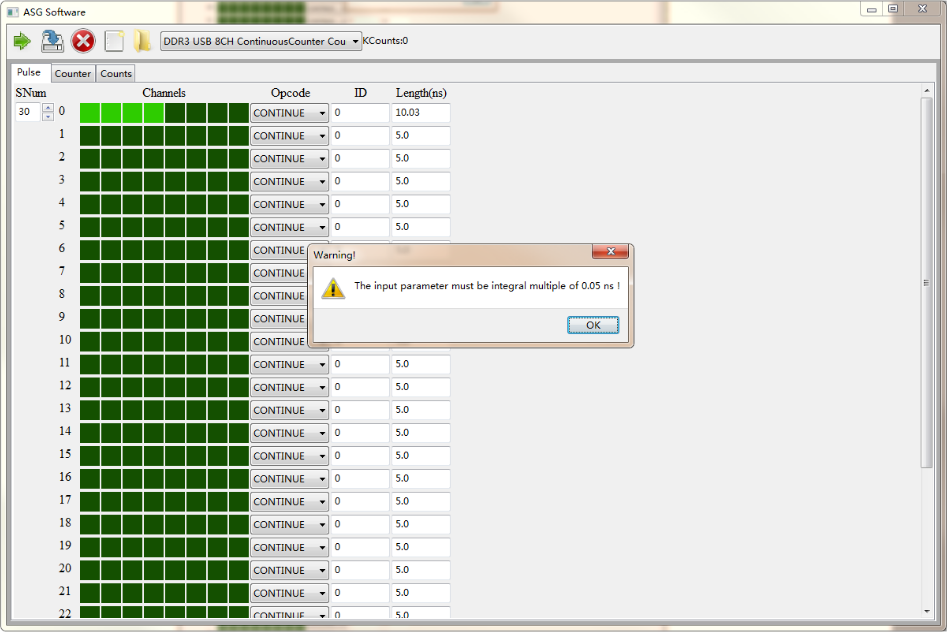
\includegraphics[width=11cm,height=9cm]{fig4_5}
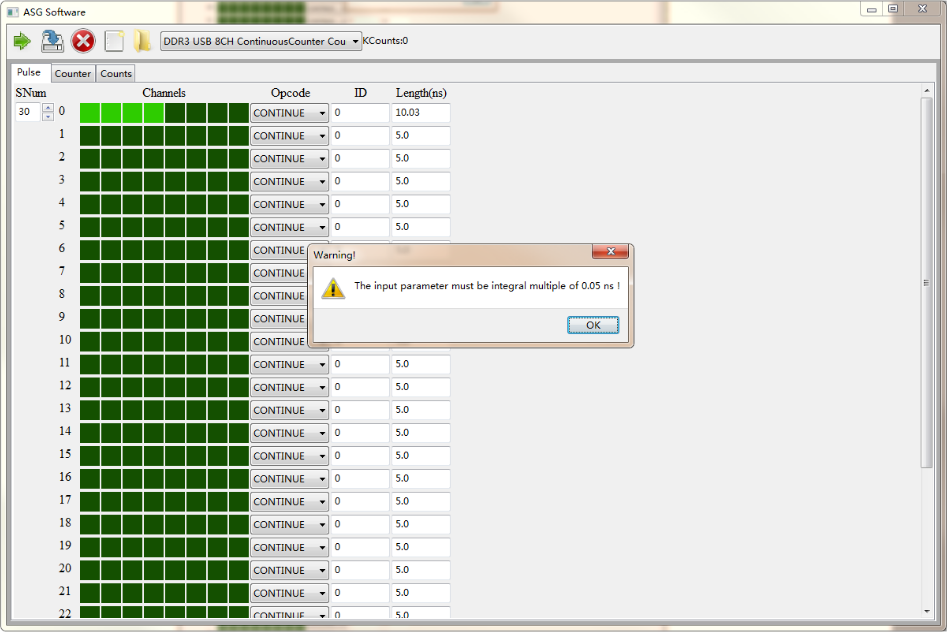
\includegraphics[height=9cm]{fig4_5}
\caption{宽度不是0.05 ns整数倍的非法方波序列输入}
\end{figure}

\section{\heiti 开始播放方波序列}
用户点击“Download”按钮

\includegraphics{download},可将自定义方波序列数据下载到硬件中。点击“Start”按钮

\includegraphics{start},可使仪器各输出通道开始同步播放用户自定义的方波序列。将输出通道用同轴线连接至示波器上可以看到仪器输出的方波波形。

\section{\heiti 停止播放方波序列}
当仪器正在播放方波序列时,可以通过点击“Stop”按钮
\includegraphics{stop}使仪器停止播放方波序列。





